\chapter{Data acquisition and annotation \statusfirstdraft}
	\label{chap:data}
	
	This chapter describes the data that influenced the decisions of selecting the cell detection and tracking methods. In \cref{sec:data_examples} we briefly describe the imaging method used to acquire the image sequences and present some example datasets. \Cref{sec:data_challenges} describes some of the challenges of tracking cells in these datasets. \Cref{sec:data_tool} presents the data annotation tool that was developed to ease the annotation process.

    \section{Data acquisition and example datasets \statusseconddraft}
    \label{sec:data_examples}
    
    As discussed in the concluding section of \cref{chap:relatedwork}, the datasets heavily influenced the choice of algorithms for cell detection and tracking. Many computer vision algorithms rely on heuristics to improve their accuracy. In cell detection methods, this is obvious from the fact that a algorithm developed for a certain type of imaging method will likely perform poorly on an different types of images (e.g.\ different shape of cells). In cell tracking heuristics help adjust the algorithms to the specific behaviour of cells that are being analysed. For example, a different tracking method could be used for images with cells that move slowly (and there is a large overlap between cells in consecutive frames) than for cells that move quickly (and there is little overlap between cells in consecutive frames).
    
    The data acquisition process is not part of this research. However, for the reasons stated above, it is important to know the characteristics of the datasets. Because these are directly influenced by the imaging method, we follow by outlining the image acquisition process, and then present the datasets used in the evaluation of our methods.
    
    The image sequences that inspired the development of the methods describe in this thesis were acquired \textit{in vivo}. This means that the images are obtained on living mice, in contrast to \textit{in vitro} where cells are analysed on a tissue sample in a standard laboratory environment using petri dishes and other instruments. \textit{In vivo} analysis is preferred over \textit{in vitro} because it is better suited for observing the behaviour of cells in their natural environment.
    
    Recent advances in intravital microscopy of the lung \cite{looney11} and other organs allow us to image neutrophils and other cells of interest simultaneously by combining fluorescent reporter mice and intravenously-injected fluorescently-labelled antibodies. Briefly, the mouse is anaesthetized, mechanically ventilated and the surface of the lung is exposed surgically. Then a specialized ``vacuum chamber'' (as in \cite{looney11}) is used to stably hold a glass coverslip against the surface of the lung. The alveoli, alveolar capillaries and associated cells can then be visualized by laser scanning confocal microscopy. The same apparatus can be used to interrogate other organs without mechanical ventilation, e.g.\ the liver.
        
    All the data was provided by Dr. Leo Carlin from the Leukocyte Biology Section at the National Heart and Lung Institute (NHLI)\footnote{\url{http://www1.imperial.ac.uk/nhli/}}.
    
    \subsection{Datasets \statusseconddraft}
       
	From the datasets provided by Dr. Leo Carlin, five have been selected to use in the evaluation of this work because of their distinct characteristics. The original dimensions of the datasets were 512-by-512 pixels, but some have been cropped to reduce the number of cells that had to be annotated to train the cell detector and tracker.
	
	Below we describe the main characteristics of the datasets, together with the number of frames that were annotated to train the cell detector. Because of the large number of trajectories in certain datasets, not all the trajectories have been annotated. Instead, in each dataset a few trajectories were chosen and annotated. We aimed to select the longest trajectories, as these could give the most insight in the analysis of cell behaviour.
	
	\subsubsection{Dataset A}
	\label{subsec:datasetA}
	\todo[inline]{This is series30green}
	\begin{figure}[h]
   		\begin{subfigure}{.32\textwidth}
   		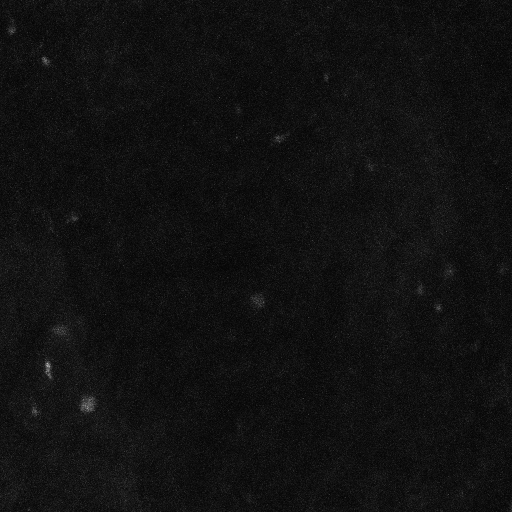
\includegraphics[width=\textwidth]{images/series30green019}
   		\end{subfigure}%
   		\hfill
   		\begin{subfigure}{.32\textwidth}
   		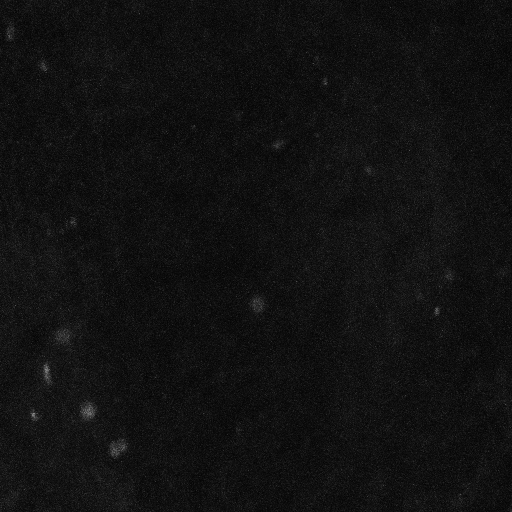
\includegraphics[width=\textwidth]{images/series30green020}
   		\end{subfigure}
   		\hfill
   		\begin{subfigure}{.32\textwidth}
   		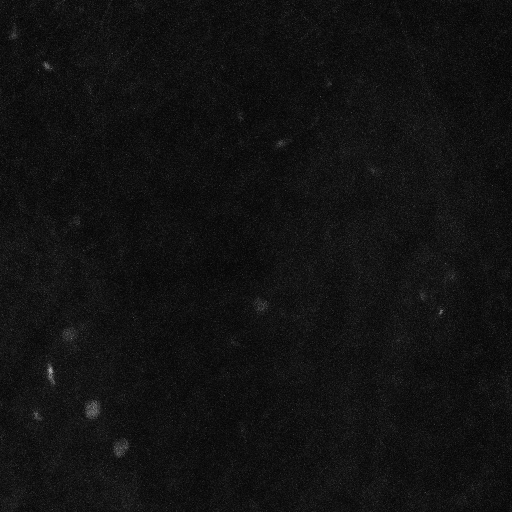
\includegraphics[width=\textwidth]{images/series30green021}
   		\end{subfigure}
   		\caption{Three consecutive frames from dataset A.}
   		\label{fig:data_datasetA}
   	\end{figure}
   	  	
   	Dataset A, seen in \cref{fig:data_datasetA}, contains 66 frames of dimensions 512-by-512 pixels. All the frames have been manually annotated for the purpose of training the cell detector. The dataset only has an average population of 1.58 cells per frame, and all four main trajectories have been annotated, although three of them can only be tracked in a dozen frames. The dataset is obtained from the liver. There is a good contrast between the cells and the background. The background is almost uniform but still contains some information about the architecture of the liver sinusoids, which is difficult to discern without adjusting the image contrast. The cells appear as medium dark shades of grey of circular shape and their boundaries smoothly blend with the background. The cells move slowly. Despite the small number of frames, this is an especially challenging dataset for the cell detection module. Frames 1--17 are radically different from frame 18 and onwards. The first 17 frames show little contrast between the cells and the background. On frame 18, the images change such that the texture from the background becomes very similar to the texture of the cells in the first 17 frames, and the intensity of the cells intensifies. Finally, the last few frames contain no cells.
   	   	
	\subsubsection{Dataset B}
	\todo[inline]{This is series30red}
	\begin{figure}[h]
		\begin{subfigure}{.32\textwidth}
		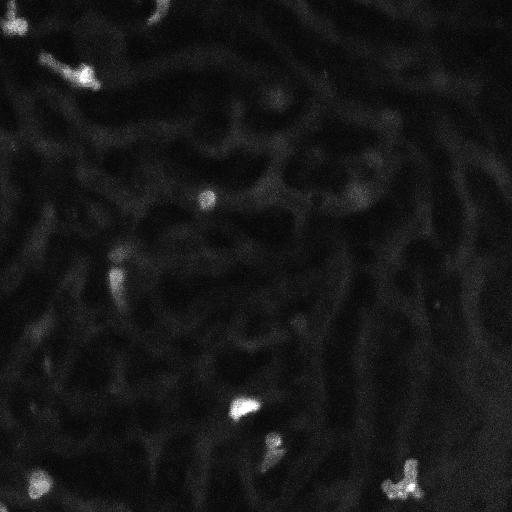
\includegraphics[width=\textwidth]{images/series30red024}
		\end{subfigure}%
		\hfill
		\begin{subfigure}{.32\textwidth}
		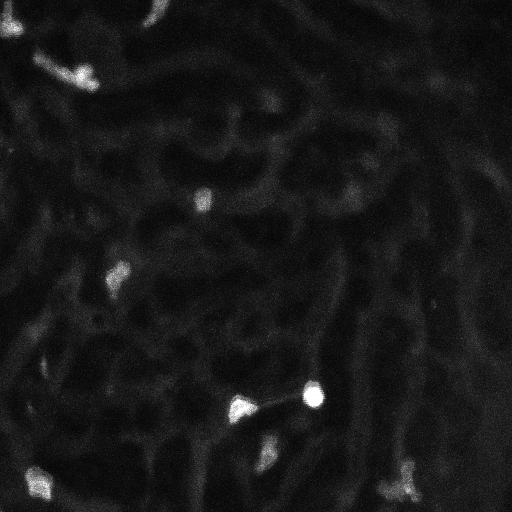
\includegraphics[width=\textwidth]{images/series30red025}
		\end{subfigure}
		\hfill
		\begin{subfigure}{.32\textwidth}
		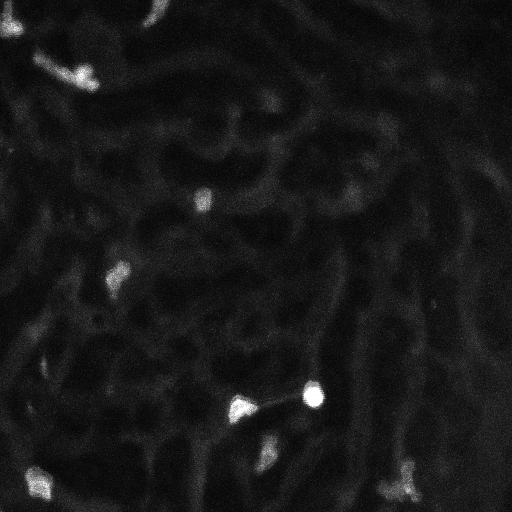
\includegraphics[width=\textwidth]{images/series30red025}
		\end{subfigure}
		\caption{Three consecutive frames from dataset B.}
		\label{fig:data_datasetB}
	\end{figure}
		
	\Cref{fig:data_datasetB} shows three consecutive frames from dataset B. The dataset contains 66 frames of dimensions 512-by-512 pixels and an average population of 8.03 cells per frame. The entire dataset has been annotated for the purpose of training the cell detector and (TODO ~5) of the longest trajectories for the purpose of training the cell tracker. This dataset is also obtained from the liver sinusoids. The cells appear brighter than in dataset A, but their shapes vary. Some are round and others elongated and deformed to fit into the tight liver sinusoids in which they move. Their brightness varies from medium to very bright. The brighter ones have clearer boundaries than the medium bright ones, whose boundaries are softer. In the background we can clearly discern the blood vessels in a darker grey colour. Cells in this dataset are active. Some move relatively fast and change direction frequently. The images are of constant quality, and there are few significant camera artefacts.

	Although datasets A and B were obtained simultaneously, cells in dataset A were marked with a fluorescent reporter (green fluorescent protein -- GFP) that the mouse has been genetically modified to produce just in a type of immune cells termed 'NK' cells, while those in dataset B were diffusely staining (unbound Ab in circulation), which is weaker and colours the cells more diffusely.
	
	\subsubsection{Dataset C}
	\todo[inline]{This is series13greencropped}
    \begin{figure}[h]
    	\begin{subfigure}{.32\textwidth}
    		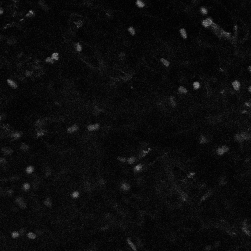
\includegraphics[width=\textwidth]{images/series13greencropped008}
    	\end{subfigure}
    	\hfill
    	\begin{subfigure}{.32\textwidth}
	    	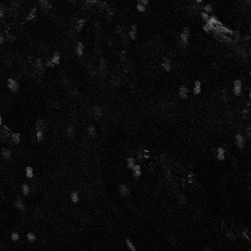
\includegraphics[width=\textwidth]{images/series13greencropped009}
    	\end{subfigure}
   		\hfill
  	    \begin{subfigure}{.32\textwidth}
   	  		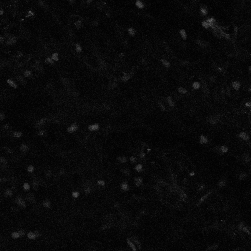
\includegraphics[width=\textwidth]{images/series13greencropped010}
  	    \end{subfigure}
    	\caption{Three consecutive frames from dataset C.}
    	\label{fig:data_datasetC}
    \end{figure}
        
    Dataset C, seen in \cref{fig:data_datasetC}, is composed of 126 frames which have been cropped to 251-by-251 pixels. The first 58 frames have been annotated with dot-annotation for the purpose of training the cell detector, and 5 of the longest trajectories were annotated for the purpose of training the cell tracker. This dataset is also obtained from the lung. The dataset contains an average population of 19.45 cells per frame as estimated from the annotated frames. The background is dark, but contains several very faint cells which we are not interested in tracking. We are interested in tracking the brighter cells. The colours of the cells are dark to medium grey. The cell boundaries blend smoothly with the background. Most cells appear as round patches. Although the cells are mostly stagnant, but the lung tissue is moving due to the breathing of the mice. For this reason, the dataset contains many motion artefacts. Some frames are blurred, and many appear to contain the duplicates of the cells shifted in position by a small amount, as seen in the middle image in \cref{fig:data_datasetC}.

	\subsubsection{Dataset D}
	\label{sec:datasetD}
	\todo[inline]{This is series14croppedclean}
	\begin{figure}[h]
		\begin{subfigure}{.32\textwidth}
		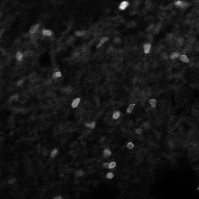
\includegraphics[width=\textwidth]{images/series14croppedclean024}
		\end{subfigure}%
		\hfill
		\begin{subfigure}{.32\textwidth}
		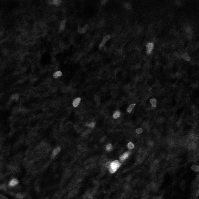
\includegraphics[width=\textwidth]{images/series14croppedclean025}
		\end{subfigure}
		\hfill
		\begin{subfigure}{.32\textwidth}
		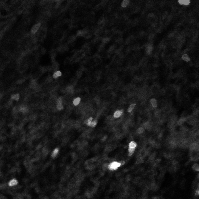
\includegraphics[width=\textwidth]{images/series14croppedclean027}
		\end{subfigure}
		\caption{Three consecutive frames from dataset D.}
		\label{fig:data_datasetD}
	\end{figure}

 	Dataset D, seen in \cref{fig:data_datasetD}, is likely to be the most challenging for the tracking module. It was originally composed of 682 frames. Unfortunately, the dataset contained large sequences of frames that were of exceptionally low quality, such that even a human could not track the cells accurately. Thus, the dataset has been manually pruned to 377 frames and cropped to dimensions 199-by-199 pixels. 53 frames have been annotated with dot-annotations and 7 of the longest trajectories. Dataset D is obtained from the lung. The cell density is 10.32 cells per frame. The background contains some noise, but it is still relatively different to the texture of the cells. The cells are mostly elliptical and have a strong boundaries. This dataset contains several fast moving cells. As mentioned before, the dataset contains many motion artefacts, the contrast of the images is constantly changing, and often about half of the cells in each frame become invisible for a few frames, even after manually eliminating the most affected.
	
	\subsubsection{Dataset E}
	\todo[inline]{This is seriesm170\_13cropped}
	\begin{figure}[h]
	
		\begin{subfigure}{.32\textwidth}
		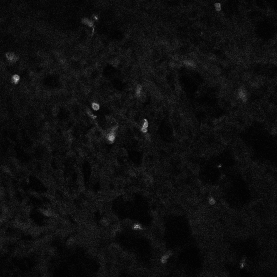
\includegraphics[width=\textwidth]{images/seriesm170_13cropped016}
		\end{subfigure}%
		\hfill
		\begin{subfigure}{.32\textwidth}
		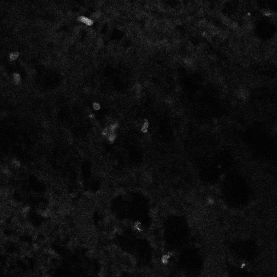
\includegraphics[width=\textwidth]{images/seriesm170_13cropped017}
		\end{subfigure}
		\hfill
		\begin{subfigure}{.32\textwidth}
		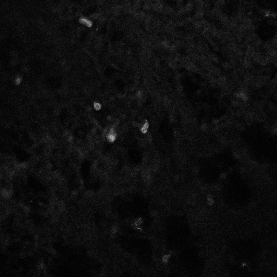
\includegraphics[width=\textwidth]{images/seriesm170_13cropped018}
		\end{subfigure}
		\caption{Three consecutive frames from dataset E.}
		\label{fig:data_datasetE}
	\end{figure}
        
    The last dataset, seen in figure \cref{fig:data_datasetE}, contains 194 frames which have been cropped to dimensions 277-by-277 pixels. 67 frames were annotated for the purpose of training and evaluating the quality of the cell detection module. (TODO) of the longest trajectories were annotated for training the tracker. This dataset is from the lung. The density of the cells is of $7.01$ cells per frame. The background contains some texture, that could sometime be confused with the cell texture. The cells in this dataset appear smaller than in the other datasets and are less elliptical. They contain more sharp edges. The intensity of the cells varies from dark to bright. The cells appear to move very slowly. The images contain many artefacts that make tracking more difficult. First, the images become darker in towards the middle of the image sequence, and then close to the last quarter of the sequence become clear again. Second, there is an alternating dark/bright area in all the frames caused by the raster scanning imaging method combined with the moving tissue.
    	
	\subsection{Image analysis challenges \statusseconddraft}
	\label{sec:data_challenges}
	In this section we are going to present two phenomena caused by the combination of moving tissue due to ventilation and a raster scanned image that make these datasets especially hard to track with frame-by-frame tracking methods.
	
	The first challenge are the artefacts caused by the scanned image. They appear as alternating dark/bright horizontal lines which seem to move from the top to the bottom of the images. The effect can be seen in \cref{fig:data_challenge_shutter}. This makes the tracking problem difficult, because the cells behind the dark areas appear fainter or disappear completely for the few frames that they are covered.
		
	\begin{figure}[h]
	
		\begin{subfigure}{.32\textwidth}
		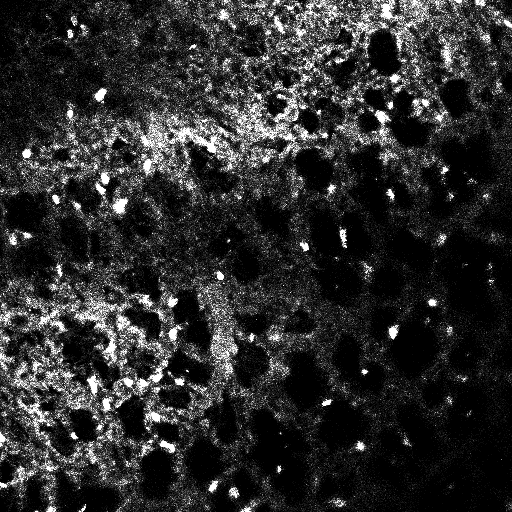
\includegraphics[width=\textwidth]{images/shutterseriesm170_13cropped001}
		\end{subfigure}%
		\hfill
		\begin{subfigure}{.32\textwidth}
		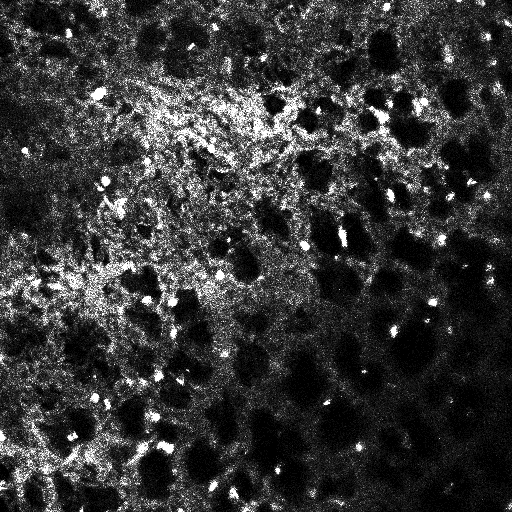
\includegraphics[width=\textwidth]{images/shutterseriesm170_13cropped002}
		\end{subfigure}%
		\hfill
		\begin{subfigure}{.32\textwidth}
		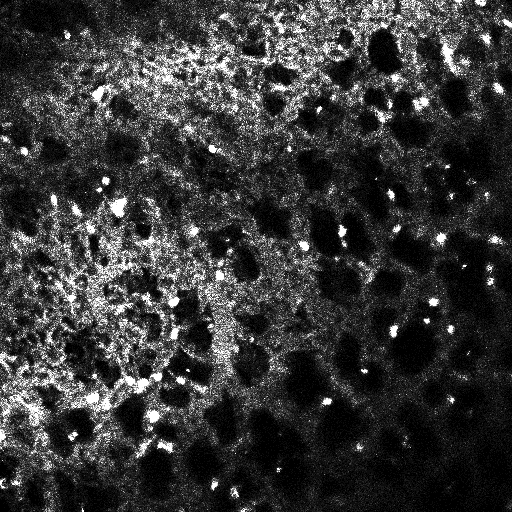
\includegraphics[width=\textwidth]{images/shutterseriesm170_13cropped003}
		\end{subfigure}%
		\vspace{0.3cm}
		\begin{subfigure}{.32\textwidth}
		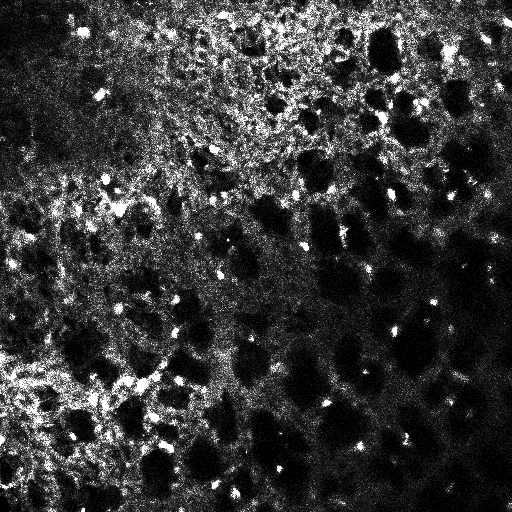
\includegraphics[width=\textwidth]{images/shutterseriesm170_13cropped004}
		\end{subfigure}%
		\hfill
		\begin{subfigure}{.32\textwidth}
		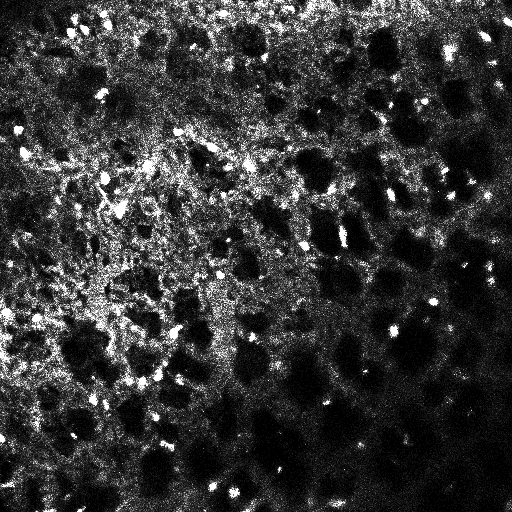
\includegraphics[width=\textwidth]{images/shutterseriesm170_13cropped005}
		\end{subfigure}%
		\hfill
		\begin{subfigure}{.32\textwidth}
		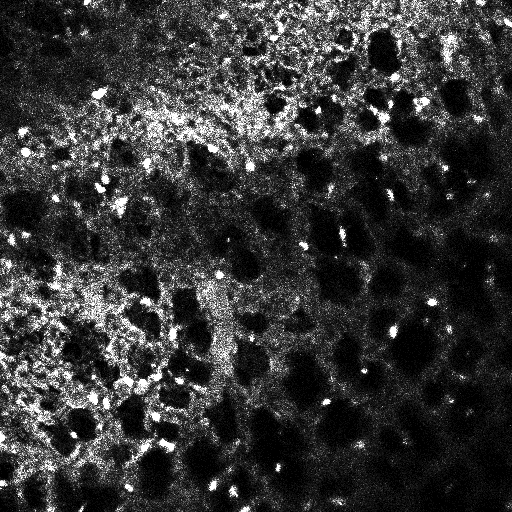
\includegraphics[width=\textwidth]{images/shutterseriesm170_13cropped006}
		\end{subfigure}
		\caption{Six consecutive frames from a sequence displaying the alternating dark/bright regions caused by the camera shutter. The contrast and sharpness of the images has been adjusted to dramatize the effect.}
		\label{fig:data_challenge_shutter}
	\end{figure}
	
	The second challenge is the movement of the tissue, especially in the case of lung imaging. The shaking can be in the x-y plane, but sometimes, as in the case shown in figure \cref{fig:data_challenges_movement} it can be primarily in the z-direction. Displacement in the x-y direction causes the cells to jiggle. Displacement of the tissue in the z-direction causes part of all of the image to become out-of-focus for a few frames.
	
	\begin{figure}[h]

		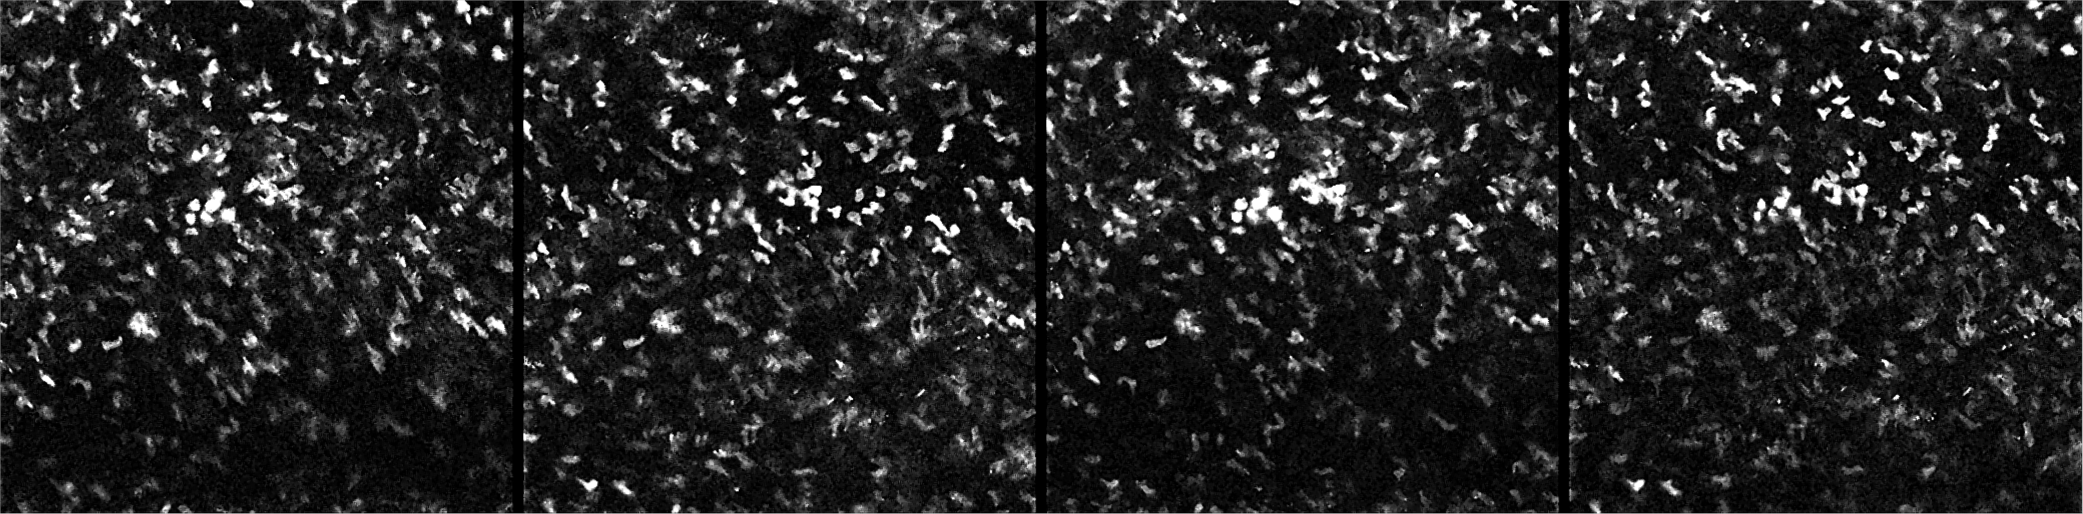
\includegraphics[width=\textwidth]{images/data_challenge_movement}

		\caption{Four consecutive frames taken from the lung displaying varying cell clarity due to the displacement caused by the lung movement. The contrast of the images has been adjusted to dramatize the effect.}
		\label{fig:data_challenges_movement}
	\end{figure}
	
	Several of the datasets present these phenomena to a lesser or larger extend. These artefacts where the primary reason for choosing a global optimization method for associating detection responses into trajectories instead of a frame-by-frame approach.
	
	\subsection{Manual data annotation \statusnew}
	
	Training the detector requires a set of annotated image sequences. Precise and consistent dot-annotations allow the model to learn well. Precise annotations are those where the annotation dots are place within the actual cell. If the dot-annotation is placed on the near, yet outside of cell, the detector will incorrectly learn to discriminate cells from the background. Consistent annotations are those where the annotator takes special care to annotate cells that look alike. For example, if only bright cells are annotated in one frame, but bright and dark cells in the next frame, the detector will not be able to reliable detect both bright and dark cells.
	
	The major challenge of annotating the datasets is consistency, due to the human ability to easily identify cells from the background, even if their relative intensities vary significantly. The detection module is able to learn well even with the presence of a few outliers.
	
	It was important to correctly annotated a certain number of frames on each dataset. Annotating the entire datasets would represent a lot of unnecessary manual work, because the detector can be trained on just a few dozen annotated frames. We have manually annotated and reviewed about 50 frames from each dataset. The counts of annotated frames and cell density metrics are presented in \cref{tab:results_data_count}.

	\begin{table}[h]
		\centering
		\begin{tabular}{rp{3cm}p{3cm}p{3cm}p{4cm}}
			Dataset & Number of annotated frames & Number of annotated cells & Average number of cells per annotated frame & Standard deviation of number of cells per annotated frame \\
		\hline
			      A &    66   &   104 &   1.58  &    0.86  \\
			      B &    66   &   530 &   8.03  &    2.44  \\
			      C &    58   &  1128 &  19.45  &    4.19 \\
			      D &    53   &   547 &  10.32  &    2.54 \\
			      E &    67   &   470 &   7.01  &    2.25 
		\end{tabular} 
		\caption{
			Summary of the number of frames and cells manually annotated in each dataset.}
		\label{tab:results_data_count}
	\end{table}
	
	In the next section we present the tool developed to facilitate the annotation process.

    \section{The annotation tool \statusfirstdraft}
    \label{sec:data_tool}
    	In order to train the cell detector and tracker it is necessary to annotate a few frames from the datasets. The cell detector requires dot annotations - a single dot within each cell - that indicate whether an extremal region corresponds to a cell. The detector is then trained to recognize extremal regions similar to the ones that were annotated. Similarly, the cell tracker needs annotations that indicate whether two cells from different frames belong to the same tracklet. The cell tracker is then trained based on the similarity of the appearance and spatio-temporal features extracted from these cells.
    	
    	To train a good detector and tracker it is important that the annotations are consistent. For example, several datasets contain cells that appear bright and some that are darker. If we are only interested in tracking the cells that consistently appear bright, the annotations should only include the bright cells. The models may not be trained correctly if only part of the bright cells were annotated. Note that this paragraph makes observations about brightness because the concept is easy to understand for a reader. However, the detector and tracker rely on many more features for detection and tracking.
	
		To facilitate the annotations of datasets a new annotation tool has been developed. The graphic user interface of the tool is visible in \cref{fig:data_annotator_screenshot}. The tool is able to load a sequence of images, display them and permits the user to annotate them. The user is able to preform the following actions: adding a dot detection, deleting a dot detection, adding a link between cells, deleting a link between cells. The tool also features zooming and panning.
		

		\begin{figure}
			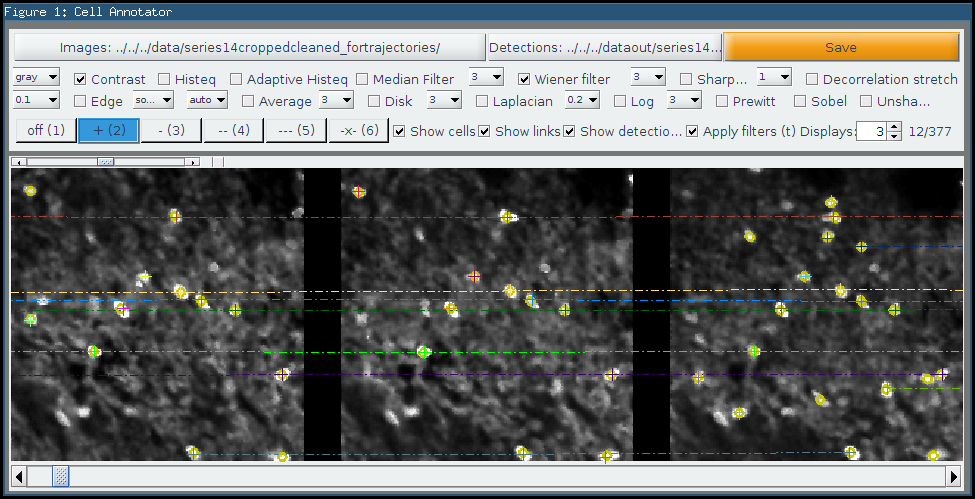
\includegraphics[width=\textwidth]{images/data_annotator_screenshot}
			\caption{Screenshot of the annotation tool. User annotations are shown as crosses and dashed links between them, while detection responses are are shown as yellow circles.}
			\label{fig:data_annotator_screenshot}
		\end{figure}
		
		\begin{figure}
			\centering
			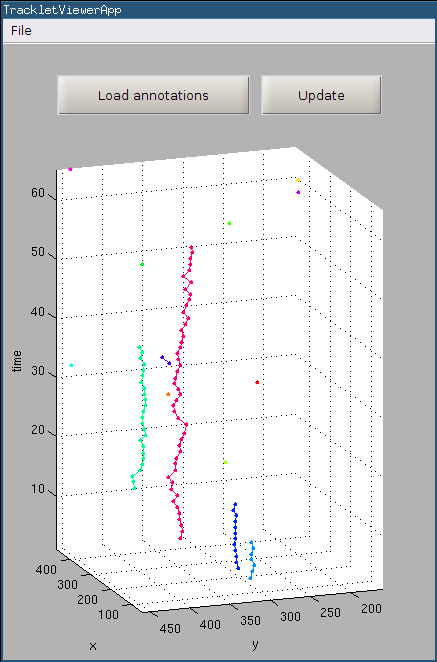
\includegraphics[width=.48\textwidth]{images/data_tracklet_viewer}
			\caption{Screenshot of the interactive 3D tracklet viewer showing annotations for Dataset A.}
			\label{fig:data_tracklet_viewer}
			
		\end{figure}
				
						
		Furthermore, the tool includes a broad set of filters that can be applied on the images to increase the clarity of the cells and ease the annotation process. These filter include contrast adjustments, smoothing, sharpening, edge detection, etc. To reduce the clutter on densely populated datasets, the user is able to only display annotations from a specific part of the image, hide trajectories that include more than three dot annotations, hide the part of the GUI containing the buttons and filters in order to focus on just the images (\textit{full-screen mode}), and more.
		
		The annotation tool includes detection of potentially bad annotations. These include a warning system that displays a triangle next to a cell if two annotations are very close together and a different display style for links that deviate too much from the average (in terms of between-frame displacement). These help the eliminate accidental human errors, that would be very hard to discover otherwise.


		Finally, the tool can also be used to compare the detection responses obtained from the cell detector by overlaying them over the images. In \cref{fig:data_annotator_screenshot} these detections are shown as yellow circles. This can be very useful to visually evaluate the quality of the detections, and possibly reveal cells that the user might have missed when annotating.
		

		In addition to the annotation tool, another small GUI has been developed that shows the annotations in an interactive 3D view, where each tracklet colour is different. This tool is shown in image \cref{fig:data_tracklet_viewer}. It is helpful to recognize possibly bad annotations (for example an outlier cell within a trajectory) or discover missed links.
		
		All the annotations have been reviewed by Dr. Leo Carlin, who provided the datasets. However, due to the noisy nature of the images, some of the dataset are difficult to correctly annotate even for a human. It is expected that a small number of annotations are erroneous.
		
		Both tools were developed and packaged as standalone executables with MATLAB 8.3.0.532 (R2014a). The tools do not depend on MATLAB to run, but require the free MATLAB Compiler Runtime 8.3\footnote{\url{http://www.mathworks.co.uk/products/compiler/mcr/}} which is automatically downloaded and installed when the applications are installed on the system. Installation guides for both applications are provided in appendices \ref{app:annotationtool} and \ref{app:interactiveviewer}.